%% Copernicus Publications Manuscript Preparation Template for LaTeX Submissions
%% ---------------------------------
%% This template should be used for copernicus.cls
%% The class file and some style files are bundled in the Copernicus Latex Package, which can be downloaded from the different journal webpages.
%% For further assistance please contact Copernicus Publications at: production@copernicus.org
%% https://publications.copernicus.org/for_authors/manuscript_preparation.html


%% Please use the following documentclass and journal abbreviations for preprints and final revised papers.

%% 2-column papers and preprints
\documentclass[esurf, manuscript]{copernicus}

\usepackage{makecell}
\usepackage{float}
\usepackage[section]{placeins}
 
\newcommand{\aref}[1]{\textbf{Reference #1}}
\newcommand{\afig}[1]{\textbf{Figure #1}}
\newcommand{\TODO}[1]{\textbf{TODO: \color{red}#1}}
\newcommand{\ian}[1]{{\textbf{\color{blue}Ian sayz:} \color{blue} #1} }
\newcommand{\mauro}[1]{{\textbf{\color{green}Mauro says:} \color{green} #1} }
\newcommand{\alpine}{\textit{ALPINE}}
\newcommand{\icesheet}{\textit{ICESHEET}}
\newcommand{\m}{$\,\mathrm{m}$\,}
\newcommand{\cm}{$\,\mathrm{cm}$\,}
\newcommand{\mma}{$\,\mathrm{mm  \, a^{-1}}$\,}
\newcommand{\mmma}{$\,\mathrm{m^3\, a^{-1}}$\,}
\newcommand{\mmms}{$\,\mathrm{m^3\, s^{-1}}$\,}
%\newcommand{\unit}[1]{$\mathrm{#1}$}

\begin{document}

\title{Subglacial and subaerial fluvial sediment transport capacity respond differently to water discharge variations}

% \Author[affil]{given_name}{surname}


\Author[1][IanArburua.Delaney@unil.ch]{Ian}{Delaney} %% correspondence author
\Author[2]{Andrew J.}{Tedstone}
\Author[3,4]{Mauro A.}{Werder}
\Author[3,4]{Daniel}{Farinotti}

\affil[1]{Institut des dynamiques de la surface terrestre (IDYST), Universit\'{e} de Lausanne, B\^{a}timent G\'{e}opolis, 1015 Lausanne, Switzerland}
\affil[2]{Department of Geosciences, University of Fribourg, Ch. du Musée 1700, Fribourg, Switzerland}
\affil[3]{Laboratory of Hydraulics, Hydrology and Glaciology (VAW), ETH-Z\"urich, H\"onggerbergring 26, 8093 Z\"urich, Switzerland}
\affil[4]{Swiss Federal Institute for Forest, Snow and Landscape Research (WSL) Z\"uricherstrasse 111, 8903 Birmensdorf, Switzerland}
%% The [] brackets identify the author with the corresponding affiliation. 1, 2, 3, etc. should be inserted.

%% If an author is deceased, please mark the respective author name(s) with a dagger, e.g. "\Author[2,$\dag$]{Anton}{Smith}", and add a further "\affil[$\dag$]{deceased, 1 July 2019}".

%% If authors contributed equally, please mark the respective author names with an asterisk, e.g. "\Author[2,*]{Anton}{Smith}" and "\Author[3,*]{Bradley}{Miller}" and add a further affiliation: "\affil[*]{These authors contributed equally to this work.}".

\runningtitle{Subglacial sediment transport capacity}

\runningauthor{Delaney et al.}
\received{}
\pubdiscuss{} %% only important for two-stage journals
\revised{}
\accepted{}
\published{}

%% These dates will be inserted by Copernicus Publications during the typesetting process.


\firstpage{1}

\maketitle

\begin{abstract}
  Sediment transport capacity in both subaerial and subglacial channels depends on the shear stress exerted across the channel bottom, which varies with water velocity and channel width.
  In subaerial channels, water discharge variations are accommodated  by flow depth and width changes, along with water velocity.
  However, in subglacial channels,  water discharge changes mainly result in velocity variations, as the channel geometry evolves slowly (over days).
  Here, we present relationships between water discharge and sediment transport under several channel types.
  They demonstrate that sediment transport is highly non-linear with respect to water discharge with fixed subglacial channel size, and in fact can very less that subaerial flow if water discharge changes slowly enough to be in equilibrium with subglacial channel size.
  We then apply hydrographs from an Alpine glacier and the Greenland Ice Sheet to subglacial and subaerial hydraulics models, revealing greater variability in the inferred sediment transport capacity in subglacial than in subaerial channels, as subglacial channels evolve in size.
  This variability stems from the slowly evolving channel size that forces water velocity to accommodate variations in water discharge.
  Furthermore, the changing channel size means that sediment transport capacity peaks prior to the maximum water discharge.
  Results also show that high subglacial sediment transport rates and water velocities can occur across a wide range of water discharges, meaning that in a transport-limited system there could be a variable relationship between sediment and water discharge.
  These findings are discussed in the context of understanding sediment discharge from glaciers with different hydro-climatic forcings and assumptions of channel shape.
  We also examine the implications for interpreting records of sediment discharge in glacierized catchments
\end{abstract}


\introduction  %% \introduction[modified heading if necessary]

Changes in glacier dynamics and hydrology  have prompted numerous  recent studies of  sediment transport processes in cold regions \citep[e.g.][]{li2022,vergara2022,zhang2022}.
Increases in sediment transport  have been observed in Greenland \citep{bendixen2017}, the European Alps \citep{costa2017}, the Himalayas \citep{li2021}, and the Andes \citep{vergara2022}.
To explain observed changes to sediment transport in glacierized catchments requires examining the processes controlling sediment discharge and its variations with water discharge  \citep[e.g.][]{riihimaki2005,swift2005}.

Periods of millennia or longer, processes such as glacier abrasion and quarrying sculpt landscapes and create sediment to be transported fluvially from under glaciers \citep[c.f.][]{hallet1979,iverson2012,ugelvig2018}.
Pressurized subglacial water can transport this sediment from underneath glaciers \citep{walder1994,creyts2013,beaud2018,delaney2019}, if it is reachable by the water.

In a transport-limited regime, sediment discharge is controlled by sediment transport capacity, defined as the amount of sediment the water can carry.
In both subglacial and subaerial channels, sediment transport capacity depends on the shear stress between water and the sediment it flows  over \citep{shields1936,meyer1948,engelund1967} along with the width of the channel bottom $w$ over which sediment mobilizes.
The shear stress $\tau$ responds to the velocity of water $v$ flowing through the channel so that
\begin{linenomath*}
  \begin{equation}
    \label{eq:tau}
    \tau \propto v^2.
  \end{equation}
\end{linenomath*}
% 
Following mass conservation, the mean velocity of the water flowing through a  channel is
\begin{linenomath*}
  \begin{equation}
    \label{eq:v}
    v = \frac{Q}{S},
  \end{equation}
\end{linenomath*}
where $Q$ is water discharge,  and $S$ is the channel's wetted area. 

In subaerial channels, operating with open channel flow, the wetted area $S$ of the channel evolves with changing water discharge $Q$, by changing both the channel's width and the water depth \citep{leopold1953}.
The change in water depth results in a proportional increase in water velocity, and  the shear stress $\tau$ increases according to Equation~\ref{eq:tau}.

The response of water velocity to changing water discharge in subglacial channels differs from subaerial ones.
The size of subglacial channels is controlled by the opposing processes of channel opening by frictional heating of water flow on the one hand versus creep closure by ice flow on the other \citep{rothlisberger1972}.
As a result, the subglacial channel size only evolves relatively slowly over days, whereas water discharge can vary more quickly over hours \citep[e.g.][]{iken1986,andrews2014,nanni2020}.
Therefore, on short periods, subglacial water flow behaves more like pipe flow, and changes in water discharge $Q$ are mainly accommodated by changing water velocity $v$ \citep[Equation~\ref{eq:v} and Figure~\ref{fig:cartoon}; ][]{alley1997}.

\begin{figure}[hbt!]
  \centering
  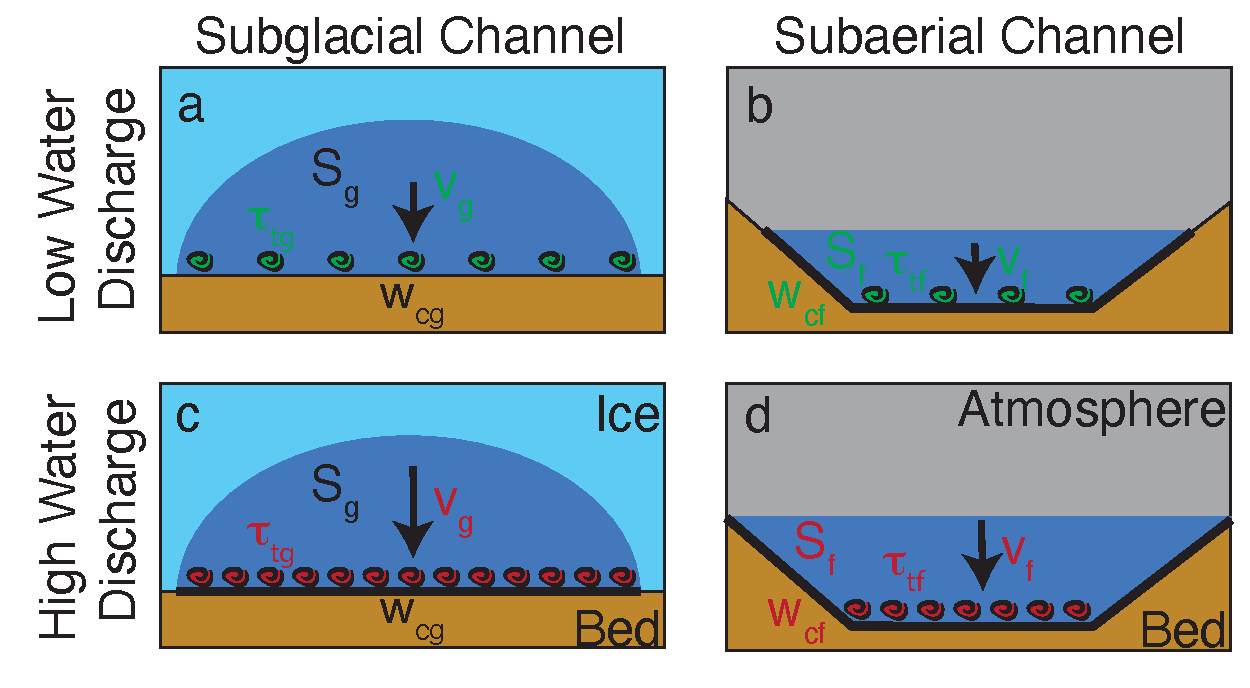
\includegraphics[width=0.6\linewidth]{Fig1.pdf}
  \caption{Sketch for the different responses of subglacial and subaerial channels to increased water discharge over short time-scales.
    Arrow length denotes water velocity magnitudes in the subglacial (subaerial) $v_g$ ($v_f$) channels.
    $S_g$ ($S_f$) represents the wetted area in subglacial (subaerial) channels.
    The subglacial channel width $w_g$ remains unchanged, while the subaerial channel width $w_f$ evolves with water discharge.
    Subglacial (subaerial) shear stress $\tau_g$ ($\tau_f$) is responsible for the mobilization of sediment.
  }
  \label{fig:cartoon}
\end{figure}

Sediment mobilization in subaerial and subglacial channels, therefore, responds differently to changing water discharge.
These differences are implicitly included in a range of models quantifying sediment transport in both subglacial and subaerial channels  \citep[e.g.][]{walder1994,alley1997,tucker1997,creyts2013,beaud2018,delaney2019,hewitt2019,wickert2019}.
To date, explicit parameterizations of subglacial sediment transport capacity with respect to water discharge has assumed fixed channel size and demonstrates a very non-linear response in sediment transport capacity to water discharge \citep{alley1997}.
The modeling frameworks examining subglacial sediment transport with evolving channel size minimally discuss the impact of different hydrological forcing on sediment transport capacity with the aim of understanding the impact of hydro-climatic conditions on subglacial sediment dynamics \citep{creyts2013,beaud2018,delaney2019,hewitt2019}.
Yet, sediment discharge capacity controls the mobilization and deposition of sediment, making it one of the most fundamental aspects of subglacial sediment evacuation, especially over short timescales.

Despite the physical differences between the subaerial and subglacial systems, water discharge and sediment export are often compared in contemporary glacial environments \citep[e.g.][]{willis1996,pearce2003,richards2003,swift2005,chu2009,tedstone2012,chu2012,overeem2017,delaney2018,swift2021,lu2022,andresen2024}.
These comparisons are natural given that the majority of sediment evacuated from glaciers over contemporary seasonal timescales is done so fluvially \citep[e.g.][]{collins1989, riihimaki2005,delaney2024}.
In subaerial systems, water discharge and sediment transport capacity for a grain size are closely linked \citep[e.g. ][]{schmidt2006,pitlick2021} \ian{check citiation}.
However, the potential for a highly variable response in sediment transport capacity in subglacial sediment transport may affect the interpretation of sediment transport records in glacial systems \citep[e.g.][]{ganti2016,mancini2023}, if properties associate with subaerial systems are assumed.
This relationship should be clarified as sediment dynamics change in glacierized regions along with changing hydrology, increased variability of water discharge \citep{lane2019} and extreme glacier melt  \citep[e.g.][]{cremona2023,overeem2015} that may drive high magnitude sediment transport events.

This manuscript as two objectives: 1) evaluate the variability of subglacial sediment transport capacity with evolving subglacial channels size and different hydrographs and 2) establish if subseasonal variations in water discharge can be covary with sediment transport capacity in subglacial systems.
First, to reenforce the highly variable behavior of subglacial sediment transport capacity,  we present algebric formulations of the sediment transport capacity response to water discharge in subaerial, pipe-flow and equilibrium R-channel conditions, extending the relationships presented in \citet{alley1997}.
We then use numerical models to examine  sediment transport capacity in subglacial channels that evolve in size and subaerial channels.
They are then applied to proglacial hydrological records from an Alpine glacier in Switzerland (Fieschergletscher) and  a land-terminating glacier in Greenland (Leverett Glacier).
We run models with an ensemble of parameters to evaluate the sediment transport capacity variability in subglacial channels compared to subaerial ones.
Lastly, model outputs demonstrate the particular processes that can drive variability in sediment discharge capacity in subglacial systems.
Together, these findings indicate differences in the relationships between  water discharge, channel geometry, and water velocity in the subglacial and subaerial channels.
The manuscript then uses the identified differences between the subaerial and subglacial channel types to discuss the implications for interpreting the processes driving variability in sediment transport records and the impact of these differences on sediment export from glaciers.


\section{Study sites and data}
\label{sect:ss_data}

Water discharge data is used from Alpine and ice sheet settings collected downstream of the glacier, assuming no water storage in the proglacial area.
The Alpine site (labeled \alpine{}) is  Fieschergletscher in the Swiss Alps ($46^\circ\,29'\,07''$ N, $8^\circ\,08'\,3''$ E).
The water discharge data used here was collected at a $1$\unit{min} interval from May 24, 2014, to October 10, 2014 \citep[Figure~\ref{fig:Qw}\,a][]{felix2022}.

The Leverett Glacier in Greenland (labeled \icesheet{}) serves as the ice sheet setting.
Water discharge was measured roughly $2$\unit{km} downstream from the terminus ($67^\circ\,03'\,5''$ N, $50^\circ\,12'\,59''$ W), at a $5$\,\unit{min} time interval from May 28, 2012 to August 8, 2012 \citet[][Figure~\ref{fig:Qw}\,b]{tedstone2013}.

Note that we omit analysis of suspended sediment discharge records due to the role of sediment supply in capturing variations in sediment discharge, in addition to sediment transport capacity \citep[e.g.][]{delaney2019}.

\begin{figure}[hbt!]
  \centering
  \includegraphics[width=0.8\linewidth]{Qw_plot.pdf}
  \caption{Water discharge from Fieschergletcher (\alpine) and Leverett Glacier (\icesheet).
    Note differences in variability and quantity of water discharge over the season.
  }
  \label{fig:Qw}
\end{figure}


\section{Methods}
\label{sect:meth}
The two models described below (Sections ~\ref{sect:sub_mode}~and~\ref{sect:fluv}) represent relationships amongst water discharge, water velocity, and channel geometry in both subaerial and subglacial channels (Table~\ref{table:vpm}).
Both models use the measured discharge to calculate water velocity, shear stress, and width-integrated shear stress, upon which both suspended sediment and bedload transport depend \citep[Figure \ref{fig:cartoon}; ][]{shields1936}.
Our evaluation in terms of shear stress omits the selection of a sediment transport relationship and a grain-size parameter \citep[e.g.][]{shields1936,meyer1948}.
Through this choice we also negate sorting processes 

\subsection{Subglacial channel  model}
\label{sect:sub_mode}

To evaluate the shear stress of water flowing across sediments underneath a glacier, the subglacial channel model accounts for the channel geometry and the water's velocity.
To do this, we use a lumped hydraulics model from \citet{werder2010b}, itself based upon  \citet{clarke1996}.

Here, it is assumed that the water is transported through a subglacial channel \citep[Figure~\ref{fig:cartoon}; ][]{rothlisberger1972} beneath a glacier with channel length $l$, with a flat bed and a mean thickness of $h_{ice}$.
The channel  size grows from melt due to frictional heating from water flow and closes due to the creep  of the ice.
The formulation here does not consider the englacial storage of water.
The evolution of subglacial channel size $S_g$ is given as
\begin{linenomath*}
  \begin{equation}
    \label{eq:dS_dt}
    \frac{\partial S_g}{\partial t} = C_1 \frac{Q \Delta h}{l} - C_2 \left(h_{o}-\frac{\Delta h}{2}\right)^n\,S_g,
  \end{equation}
\end{linenomath*}
\noindent where $t$ is time, $C_1= (1-\rho_wc_pc_t)\,\frac{\rho_wg}{\rho_iL}$ and $C_2=2A(\frac{\rho_wg}{n})^n$ are constants (complete values given in Table~\ref{table:vpm}), $g$ is the acceleration due to gravity, $Q$ is water discharge, $\Delta h$ is the hydraulic potential change over $l$, $h_{o}= \frac{\rho_i}{\rho_w} h_{ice}$ is the mean ice overburden pressure expressed in meter water equivalent ($\rho_w$ is density of water; $\rho_i$ is density of ice), and $n$ is Glen's n \citep{glen1955} (usually $n=3$).
The first term on the equation's right side represents the opening of the channel through frictional heating, while the following term represents the creep closure of the channel from ice deformation.


Following the Darcy-Weisbach equation, the head drop $\Delta h$ is
\begin{linenomath*}
  \begin{equation}
    \label{eq:dh}
    \Delta h \,  = l \,\frac{1}{2g} \,f_i\,\frac{v_{g}^{2}}{D_h},
  \end{equation}
\end{linenomath*}
\noindent where $f_r$ is a friction factor, $D_h$ is the hydraulic diameter, $l$ is the channel length, and $v_g=\frac{Q}{S_g}$ is the water flow speed.
% 
The hydraulic diameter $D_h$ is converted to wetted area $S_g$ with
\begin{equation}
  \label{eq:Dh2S}
  S_g= \frac{D_h^2}{2}\,\frac{(\frac{\beta}{2}+\sin \frac{\beta}{2})^2}{\beta - \sin \beta},
\end{equation}
where $\beta$ is the central angle of the circular segment that comprises the channel (the Hooke angle, \citet{hooke1990}). $\beta =\pi$ corresponds to a semi-circular channel and smaller values of $\beta$ result in shallow, wide channels.
This completes the subglacial hydraulic model which is described by the state variables $S_g$ and $\Delta h$.

The shear stress, $\tau_g$, between the water and the channel bed results from the Darcy-Weisbach formulation
\begin{equation}
  \label{eq:tau_g}
  \tau_g=\frac{1}{8}\,f_r\,\rho_w\,v_g^2,
\end{equation}
% 
where $v_g = \frac{Q}{S_g}$ is the water velocity.
% 
The width of the channel floor $w_g$ is represented as
\begin{equation}
  \label{eq:dh2wc}
  w_g = 2  \sin \frac{\beta}{2} \sqrt{\frac{2\, S_g}{\beta -\sin \beta}}.
\end{equation}
% 
This value is used to establish the integrated shear stress across the channel $w_g\tau_g$.

\subsection{Subaerial channel  model}
\label{sect:fluv}

The hydraulics parameterization presented in \citet{tucker1997} is implemented to represent the subaerial channel.
Using mass conservation and the Darcy-Weisbach relationship as well as assuming that the channel is sufficiently wide compared to its depth so that the hydraulic radius is well approximated by the flow depth,
the shear stress $\tau_f$ at the river bed is
\begin{linenomath*}
  \begin{equation}
    \label{eq:DW_tau}
    \tau_f=\frac{\rho_w\,g^{\frac{2}{3}}\,f_f^{\frac{1}{3}}}{2}\, \Big(\frac{Q}{w_f} \Big)^{\frac{2}{3}} \,\nabla z_c^{\frac{2}{3}},
  \end{equation}
\end{linenomath*}
where $\nabla z_c$ is the channel slope, and $f_f$ is the friction factor for subaerial channels \citep{tucker1997}.
Channel width $w_f$ is
\begin{equation}
  \label{eq:wcf}
  w_f = k \, Q^{\alpha},
\end{equation}
% 
where $k$ is a constant and $\alpha=\frac{1}{3}$ is a commonly chosen exponent \citep{leopold1953}.
Also following the Darcy-Weisbach, subaerial water velocity, $v_f$, is given as
\begin{equation}
  \label{eq:vf}
  v_f = \sqrt{\frac{8\,\tau_f}{f_f\,\rho_w}}.
\end{equation}
% 
As above, the width-integrated shear stress is $w_f\tau_f$.

Note that this subaerial channel model is purely algebraic, whereas the subglacial model comprises a differential equation for the evolution of $S_g$.
Thus the channel size in the subaerial model has no history dependence on the discharge $Q_w$, whereas the subglacial one does (Equation~\ref{eq:dS_dt}).

\begin{table}[hbt!]
  \centering
  \caption{Variables, parameters, and constants used in this work.
    Where two values are given, the first refers to  \alpine{}, a scenario from Fieschergletscher, and the second to a glacier marginal to the \icesheet{} a scenario from Leverett Glacier. If a second line is given, it refers to the range of values examined in the parameter search}
  \small 
  \begin{tabular}{ l  c  c c }
    Name &Symbol&  Value&Units \\
         && (\alpine{} or \icesheet{})\\
    \hline
    \textbf{Variables}  & & & \\
    Water discharge  & $Q$& & $\mathrm{m^{3}\,s^{-1}}$ \\
    Water velocity (subglacial, subaerial)  & $v$, ($v_g,\,v_{f}$)& & $\mathrm{m\,s^{-1}}$ \\
    Channel wetted area (subglacial, subaerial) &  $S_g, S_f$& & $\mathrm{m^2}$     \\
    Channel depth (subaerial) & $H$&& $\mathrm{m}$\\
    Hydraulic diameter &$D_h$&&$\mathrm{m}$\\
    Width of channel floor (subglacial, subaerial) & $w$, ($w_g,w_f$)&  & $\mathrm{m}$     \\
    Hydraulic head &$\Delta h$&& $\mathrm{m}$\\
    Hydraulic gradient &$\Psi=\frac{\Delta h}{l}$&& $\mathrm{m\, m^{-1}}$\\
    Shear stress (subglacial, subaerial) & $\tau$, ($\tau_g,\,\tau_f$) && $\mathrm{Pa \, m^{-2}}$ \\
    Stream power & $\Omega$ && $\mathrm{ kg \, m\, s^{-3}}$ \\


    \textbf{Parameters and Constants}  & & &\\
    Gravitational constant&$g$& $9.81$&$\mathrm{m\,s^{-2}}$\\
    Density of water & $\rho_w$& $1000$ & $\mathrm{kg\,m^{-3}}$ \\
    Density of ice & $\rho_i$& $900$ & $\mathrm{kg\,m^{-3}}$ \\
    Hooke angle of channel & $\beta$ & $\frac{\pi}{6}$ & \unit{rad}\\
         && ($\frac{\pi}{10}$, $\pi$) & \\
    Friction factor (subglacial, subaerial) & $f$, ($f_r$, $f_f$) &$5$ or $16$, $3$ & $\mathrm{(-)}$ \\
         && ($0.01$, $21$) & \\
    Glacier thickness &$h_{ice}$& $225$ or $740$  &\unit{m}\\
    Effective glacier thickness &$h_o$&$\frac{\rho_i}{\rho_w} h_{ice}$  &\unit{m}\\
    Effective glacier length &$l$& $7,000$ or $26,000$&\unit{m}\\
    Constant $1$ in Equation~3 &$C_1$&$2.2\times10^{-5}$&\unit{m}$^{-1}$\\
    Constant $2$ in Equation~3 &$C_2$&$3.7\times10^{-13}$&\unit{m}$^{-n}\,s^{-1}$\\
    Latent heat of fusion &$L$&$333.5 $&\unit{kJ\,kg}$^{-1}$\\
    Pressure melting coefficient &$c_t$&$7.5\times 10^{-8}$&\unit{K\,Pa}$^{-1}$\\
    Specific heat capacity of water &$c_p$&$4180$&\unit{J\,kg}$^{-1}$\unit{K}$^{-1}$\\
    Ice flow constant &$A$& $5.3\times10^{-24}$ &\unit{Pa}$^{-n}$\,$s^{-1}$\\
    Ice flow exponent &$n$& $3$ &$\mathrm{(-)}$\\
    
    Gradient of channel bed (subaerial) &$\nabla z_c$ &$0.02$& $\mathrm{(-)}$\\
    &&($.01$, $0.05$) & \\
    Subaerial channel factor & $k$ &$8$ & $\mathrm{s\,m^{-2}}$\\
    Channel geometry exponent &$\alpha$&$\frac{1}{3}$ &$\mathrm{(-)}$ \\
         &&($\frac{1}{3}$, $\frac{1}{2}$) & \\
    \hline
  \end{tabular}
  \label{table:vpm}
\end{table}

\FloatBarrier
\subsection{Implementation}
\label{sect:imp}

The models above are applied to proglacial discharge records from the Fieschergletscher (scenario \alpine{}) and the Leverett Glacier (scenario \icesheet{}).
Outputs of the models represent generalizable sediment transport characteristics from these hydrographs, rather than actual hydraulic conditions.
To generalize these scenarios, \alpine{}  is exemplified by Fieschergletscher's relatively thin ice thickness \citep[$h_{ice}$= $225$\,\unit{m}][]{grab2021}, low water discharge ($\sim\,10$\,\unit{m}$^3$\,\unit{s}$^{-1}$) and high diurnal variability in water discharge (Figure~\ref{fig:Qw}\, b).
\icesheet{}  is exemplified by Leverett glacier's  thick ice  \citep[$h_{ice}$= $700$\,\unit{m}; ][]{morlighem2017}, high water discharge ($\sim\,300$\,\unit{m}$^3$\,\unit{s}$^{-1}$)  and low diurnal variability in water discharge (Figure~\ref{fig:Qw}\, b).



The first experiment aims to characterize the variability in sediment discharge capacity in subglacial compared to subaerial channels across a range of channels slopes and  shapes, along with friction factors.
Additionally, we examine the effects of different water discharge variability by smoothing the water discharge over different periods.
The results below present water velocity ($v_g$, $v_f$), shear stress ($\tau_g$, $\tau_f$), and width-integrated shear stress ($w_g\tau_g$, $w_f\tau_f$) from the subglacial and subaerial models.
For brevity, these values together are referred to as ``model outputs'' in the text.
The subglacial model outputs are generally larger than their subaerial equivalents due to their large hydraulic gradients, thus greater sediment transport capacity would be expected in subglacial channels compared to subaerial ones \citep{alley1997}.
To evaluate variability, we subtract the model outputs from their values smoothed using daily averages,  detrending the seasonal signal (Figure~\ref{fig:Qw}).
We then calculate the variability in the model output by taking the standard deviation of this detrended time series.


The effect of channel shape, gradient and roughness is established by running the model with random parameter values of channel slope and geometry factors ($\beta$,$\nabla z_c$ and $\alpha$) and friction factors ($f_r$ and $f_f$; see Table~\ref{table:vpm} for value range).
Runs with parameter combinations are accepted if their mean subglacial water velocity over the season lies between $0.5$\,\unit{m}\,\unit{s}$^{-1}$ and $2$\,\unit{m}\,\unit{s}$^{-1}$ or if subaerial water velocity lies between $0.3$\,\unit{m}\,\unit{s}$^{-1}$ and $1.2$\,\unit{m}\,\unit{s}$^{-1}$, following measurements \citep[e.g.][]{werder2010b,magnusson2012,chandler2013}.
Additionally, to be accepted, subglacial model runs can only experience a flotation fraction ($\frac{\Delta h}{2\,h_o}$) of above $1.2$ for less than $2.5$\,\% of the run.
The initial condition of cross-sectional area $S_g$ is evaluated by applying a model spinup with repeatedly applying the maximum observed water discharge of the first $4$ days of the study until there is no change in the channel area. 

The routine runs until $100$ different parameter combinations for each water discharge smoothing period are accepted with the conditions described above.
Here, the water discharge input at a given time is the average over the smoothing period before that time, ranging from $15$\,\unit{min} up to $15$\,\unit{days}.

In the second experiment, the models are  applied to a reference test case for each glacier.
These experiments assumes  a subglacial channel with $\beta=\frac{\pi}{6}$ and a subaerial channel with $\alpha = \frac{1}{3}$ and slope of $0.02$ (Table~\ref{table:vpm}).
Both friction factors $f_r$ and $f_f$ are tuned so that reasonable water velocities \citep[$\sim\,1.6\,$\unit{m}\,\unit{s}$^{-1}$][]{werder2010b,chandler2013} occur for both \alpine{} and \icesheet{}.
%
To quantify the link between sediment transport capacity and water discharge, model outputs are compared to water discharge from the glaciers using Spearman rank correlation, which accounts for the ordering of values, but not their magnitude.
Rank correlation reduces the impact of the non-linear response of sediment transport capacity to the hydrological forcing.



\section{Results}
We first present formulations of sediment transport capacity in several channel types to build upon the analysis in \citet{alley1997}.
We then apply the models above (Section~\ref{sect:meth}) in two experiments by examining three model outputs.
Water velocity and shear stress represent the potential for sediment mobilization, and width-integrated shear stress represents a proxy for the total sediment transport capacity across the channel bed (Figure~\ref{fig:model_outs}).

\subsection{Sensitivity of sediment transport in different drainage regimes}
\label{sect:scaling}

Here three kinds of drainage regimes are examined, namely, subaerial channels, steady-state R-channels \citep{rothlisberger1972}, and pipe-flow (i.e. R-channels which do not have time to adjust their size to discharge conditions).
The evolving subglacial channel geometry presented in Section \ref{sect:sub_mode} is not considered.
Here we show the sediment transport capacity scaling with  a given water discharge and hydraulic gradient for three different transport formulas: Meyer-Peter M\"uller  \citep[MPM; ][]{meyer1948}, Engelund and Hansen \citep[EH; ][]{engelund1967}, and Bagnold \citep{bagnold1980}; additionally width-integrated shear stress is assessed, as used as proxy for sediment transport throughout the manuscript.

The following hydraulic relations are used.
The Darcy-Weisbach equation can be stated as
\begin{equation}
  \label{eq:DW}
  \Psi \propto f\frac{Q^2}{D_h S^2},
\end{equation}
with $\Psi = \Delta h / l$ the head gradient and friction factor $f$.
The shear stress and stream power are, respectively,
\begin{equation}
  \label{eq:tau-omega}
  \tau \propto f v^2 = f \left(\frac{Q}{S}\right)^2, \quad  \Omega \propto \Psi Q.
\end{equation}
% 

Sediment discharge is given by the MPM, EH and Bagnold formulations as
\begin{equation}
  Q_s \propto w\, \tau^{3/2}, \quad Q_s \propto w\, \tau^{5/2}, \quad Q_s \propto w \left(\frac{\Omega}{w}\right)^{3/2} H^{-2/3},
\end{equation}
respectively, for conditions well above the transport onset threshold.

As in Section~\ref{sect:fluv}, the  subaerial channel is assumed to have a width $w$ much greater than its depth $H$, such that $D_h\approx 4h$, and to have a constant head gradient ($\Psi$) given by the topography.
Further, it is  assumed that its width can be approximated by a relation $w \propto Q^\alpha$ (Equation~\ref{eq:wcf}) with $\alpha\in [0,1]$; typically $\alpha \approx 1/2$ (a so-called regime channel).
End members $\alpha=0$ or $\alpha=1$ correspond a  subaerial channels of constant width (a slot canyon) or depth (no natural equivalent), respectively.
% 
For a steady state R-channel, it is assumed that  $\Psi$ is constant (approximated by the gradient of the Shreve \citeyear{shreve1972} potential and that $S$ adjusts such that it is in steady state with $\Psi$ and $Q$.
Note that the R-channel model presented above in Section~\ref{sect:sub_mode} Equation~\ref{eq:dS_dt} calculates $\Psi$ from the time evolving $S_g$ via the Darcy-Weisbach Equation~\ref{eq:dh} and thus no Shreve approximation is then needed.
% Conversely, pipe flow has $S$ fixed and $\Psi$ adjusts to satisfy the given $Q$.
% 
Pipe flow like conditions occur when a R-channel is subjected to rapid discharge variations such that the channel cannot adjust its size significantly on the time scale of the discharge variations.
In this case, it is assumed that the cross-sectional area $S$ is fixed, and $\Psi$ adjusts to the specified $Q$.
For both R-channel and pipe flow, it is assumed that $D_h \propto S^{1/2}$.

With these assumptions the Darcy-Weisbach equation~\eqref{eq:DW} can be solved for the not-fixed quantity: $H$ for a  subaerial channel, $S$ for a R-channel, and $\Psi$ for pipe-flow.
Then, using equations~\eqref{eq:tau-omega}, the shear stress and stream power can be calculated.
These results are summarised in Table~\ref{tab:eqs1}.
Now width integrated shear stress and sediment transport can be calculated for all regimes and for all transport formulas.
The results of the 12 combinations are presented in Table~\ref{tab:Qs} and also in Table~\ref{tab:Qs} where the fractions in the exponents are approximately given by decimal numbers for ease of comparison.

\begin{table}[hbt!]
  \caption{Relations for hydraulic variables for the three drainage regimes:  subaerial channels, R-channel and pipe-flow.  Darcy-Weisbach equation is abbreviated with ``D-W'', and stream power with ``Stream p.''. }
  \small
  \label{tab:eqs1}
  \begin{tabular}{llllll}
    Regime & Fixed & Determined via D-W
    & Additional relations & Shear stress & Stream p.\\
           & & (Equation~\ref{eq:DW})  &  &  \(\tau \propto\) & \(\Omega \propto\)\\
    \hline
    Subaerial & \(\Psi\) & \(H \propto f^{1/3}\, Q^{2/3-2\alpha/3} \, \Psi^{-1/3}\) & \makecell{\(w\,\propto Q^\alpha\) \\ \(S=wH\) \\ \(D_h\propto H\)} & \(f^{1/3} Q^{2/3-2\alpha/3}  \Psi^{2/3}\) & \(Q\, \Psi\)\\
    R-channel & \(\Psi\) & \(S\, \propto f^{2/5}\, Q^{4/5} \, \Psi^{-2/5}\) & \(D_h\propto w \propto H \propto S^{1/2}\) & \(f^{1/5} Q^{2/5} \, \Psi^{4/5}\) & \(Q\, \Psi\)\\
    Pipe & \(S\) & \(\Psi \propto f \, Q^2\, S^{-5/2}\) & \(D_h\propto w \propto H \propto S^{1/2}\) & \(fx Q^2 S^{-2}\) & \(f\, Q^3 S^{-5/2}\)\\
  \end{tabular}
\end{table}

Table~\ref{tab:Qs} shows how the proxy $w\tau$ as well as $Q_s$ of the MPM, EH and Bagnold sediment transport formulas scale with respect to $Q$, $\Psi$ or $S$ for the three different regimes and for different $\alpha$.
Remarkably, the Bagnold formula has a negative exponent for $f$ in all but the pipe-flow regime.
The total transport formula EH gives a slightly stronger dependence on all variables as should be expected due to the larger exponent on $\tau$ of $\frac{5}{2}$ versus  $\frac{3}{2}$  for the others.
Albeit, the sediment transport response in pipe-flow for the Bagnold case is close to EH.
Conversely, the sediment transport proxies $w_g\,\tau_g$ \& $w_f\,\tau_f$ used below scale only as $Q^2$ for pipe-flow, whereas the transport scales at least with $Q^3$.
The exponent for the width scaling $\alpha$ only impacts relationship between sediment transport and water discharge in the EH relation in any meaningful way.
However, for the value of $\alpha$ around $\frac{1}{2}$ (a value appropriate for most streams), the exponent on $Q$ for EH is only slightly above what the other transport relations give.

The sediment discharge in the steady state R-channel scales very similarly to the  subaerial channel case for all relations and virtually identically for the $\alpha=0.5$ case.  However, note that the head gradients $\Psi$ are likely higher for comparable $Q$ in an ice-sheet marginal or alpine glacier setting than in a  subaerial channel, as is well described in \citet{alley1997}, and thus transport rates may still be much higher in a steady state R-channel.

Furthermore, R-channels will rarely operate in steady state as variations in discharge, in particular on the diurnal timescale or the timescale of severe rain or melting events, are too fast for such a channel to reach a steady state.
In such cases they operate more like a pipe of fixed cross-section \citep[e.g.][]{gimbert2016}.
Table~\ref{tab:Qs} shows that in such a situation, the sediment transport scales much more severely with discharge, with the exponent on $Q$ being between $3$ and $5$, compared to the other two regimes when that exponent is at most $1.7$ (Table~\ref{tab:Qs}).
Thus fluctuations of discharge on short timescales (on the order of a day) have the potential to cause conditions with very high sediment transport capacities, that are of far high magnitude than the subaerial channels.


\begin{table}[hbt!]
  \caption{Sediment transport proxy ($w\tau$) and rates for the three considered different transport formulas: MPM \citep{meyer1948}, EH \citep{engelund1967}, and Bagnold \citep{bagnold1980}.
  }
  \small
  \label{tab:Qs}
  \begin{tabular}{lllll}
    & Width \(\times \,\, \tau\) & MPM & EH & Bagnold\\
    & \(w\, \tau\) & \(Q_s \propto w\, \tau^{3/2}\) & \(Q_s \propto w\, \tau^{5/2}\) & \(Q_s \propto w^{-1/2}\, \Omega^{3/2} H^{-2/3}\)\\
    \hline
    Subaerial  & \(f^{1/3}\, Q^{2/3+\alpha/3}\,  \Psi^{2/3}\) & \(f^{1/2}\, Q \, \Psi\) & \(f^{5/6}\, Q^{5/3 - 2\alpha/3} \, \Psi^{5/3}\) & \(f^{-2/9}\, Q^{19/18-\alpha/18} \, \Psi^{31/18}\)\\
    R-channel & \(f^{2/5}\, Q^{4/5} \, \Psi^{3/5}\) & \(f^{1/2}\, Q \, \Psi\) & \(f^{7/10}\, Q^{7/5}\, \Psi^{9/5}\) & \(f^{-7/30}\, Q^{31/30}\, \Psi^{26/15}\)\\
    Pipe & \(f \, Q^2 \, S^{-1}\) & \(f^{3/2}\, Q^3 \, S^{-5/2}\) & \(f^{5/2}\, Q^5\, S^{-9/2}\) & \(f^{3/2} \, Q^{9/2} \, S^{-14/3}\)\\
  \end{tabular}
\end{table}

\FloatBarrier
\subsection{Increased variability in evolving subglacial channels occurs across a range of channel shapes, slopes  and friction values}
\label{sect:ensemble}

The first numerical experiment aims to compare the variability between the subglacial and subaerial  model outputs to a range of channel shapes, friction factors, and water discharge variability, as the subglacial channel's cross-sectional area is allowed to evolve.
Following the findings in Section~\ref{sect:scaling}, variability in subglacial sediment discharge capacity could approach that of subaerial systems, should water discharge variations be sufficienlty small or subglacial channels respond in size quickly.
For simplicity, we only examine $w\tau$, not the sediment transport formulas mentioned above.
%We have chosen to exclude the pipe flow case (Section~\ref{sect:scaling}) from analysis as it depends greatly on the choice of the subglacial cross sectional area $S_g$.

Across the range of parameters  examined (Section\,\ref{sect:imp}), variability in all model outputs remains higher in the subglacial system compared to the subaerial one for both \alpine{} and \icesheet{} (Figure~\ref{fig:multi_run}).
In some cases, the variability in subglacial model outputs is a  magnitude larger than their subaerial counterparts.
Results from  both \alpine{} and \icesheet{} scenarios show that variability in both subglacial and subaerial outputs decreases with smoothing time longer than approximately 1--5 days (Figure~\ref{fig:multi_run}), when the diurnal variations in water discharge are removed from smoothing.
In the \icesheet case, the smaller variability in model outputs compared to \alpine may in fact mean that the R-channel is in closer equilibrium between channel size and water discharge (Section~\ref{sect:scaling}).
In this case, water discharge variations would create smaller disparities in sediment transport capacity than even in subaerial cases as the subglacial channel size evolves to accommodate them (Table~\ref{tab:Qs}).


\begin{figure}[hbt!]
  \centering
  \includegraphics[width=0.9\linewidth]{multi_run_tmp.pdf}
  \caption{Standard deviation of detrended model outputs for different smoothing times with different subglacial and subaerial channel shapes and friction factors.
    Shaded areas denote the range of standard deviations from the accepted $100$ parameter combinations (Section~\ref{sect:imp}).
    Solid lines denote  the mean value of standard deviations.
    Markers show smoothing periods ($15$\,\unit{min}, $1$\,\unit{hr}, $12$\,\unit{hr}, $1$\,\unit{d}, $5$\,\unit{d}, $10$\,\unit{d}, and $15$\,\unit{d}).
  }
  \label{fig:multi_run}
\end{figure}

Across the range of parameters examined in both \alpine and \icesheet, variability in a subaerial model output did not exceed the corresponding subglacial one (Figures~\ref{fig:multi_run} and \ref{fig:params}).
Analysis of parameter values shows that in both cases, smaller values of $\alpha$, or closer to a slot-canyon, result in slightly greater variability in velocity and shear stress (Figure~\ref{fig:params}).
Yet, larger values of $\alpha$ can result in greater variability in width-integrated shear stress, as greater channel width changes increase the width-integrated shear stress, but not the shear stress. 
Additionally, steeper subaearial channel slopes result in greater variability in both shear stress and width-integrated shear stress, but only approach the variability of the subglacial channel in the \alpine case (Figure~\ref{fig:params}). 
%At steeper slopes, the alluvial  processes represented in the model (Section ~\ref{sect:fluv}) probably do not apply, as the.
We note that these parameters span a commonly accepted range of values, therefore do not anticipate a scenario where variability in the subaerial system would exceed the subglacial system with this hydrology.

Greater values of the subglacial and subaerial friction factor $f_i$ and $f_p$ result in greater variability in the  shear stress and width-integrate shear stress both cases (Figure~\ref{fig:params}), as expected given Equations~\ref{eq:tau_g} and \ref{eq:vf}.
However, more velocity variability is present in low values of $f_i$ and $f_p$. 
Low values of $f_i$ result in lower growth rates in subglacial channels (Equations~\ref{eq:dS_dt} and \ref{eq:dh}).
As a result, water velocity, as opposed to channel growth, accommodates increases in water discharge, and velocity variability increases.
Note as well that smaller values of channel factor $\beta$, creating low and broad channels, result in more variability in width-integrated shear stress.
Here, the channel width can grow more quickly in response to water discharge increases as compared to a semi-circular channel with $\beta = \pi$ (Equation~ \ref{eq:dh}).

\begin{figure}[hbt!]
  \centering
  \includegraphics[width=0.9\linewidth]{Parameter.pdf}
  \caption{Parameter values compared to variability in model outputs.
    Plots on the right (orange, light blue) correspond to the \alpine{} case. Plots on the left (brown, dark blue) correspond to the \icesheet case.
    Outputs are shown using $15$ minute smoothing time. 
  }
  \label{fig:params}
\end{figure}

\FloatBarrier
\subsection{Changing subglacial channel size drives different timing and variability in sediment transport capacity}

In the second numerical experiment defined in Section~\ref{sect:imp}, we aim to quantify the sources of increased variability in the subglacial model outputs as they exhibit different seasonal evolutions and peaks.
Examining the relationship between water discharge and the model outputs, different relationships emerge for the subaerial and subglacial cases due to the hysteresis in channel size in the subglacial model (Equation~\ref{eq:dS_dt}).
Because there is no history dependence in  subaerial channels, each water discharge value in the subaerial channel results in a unique water velocity, shear stress, and width-integrated shear stress (Section~\ref{sect:sub_mode}).
This characteristic results in a perfect rank correlation between the variables (Figure~\ref{fig:Qw_vari}).
\begin{figure}[hbt!]
  \centering
  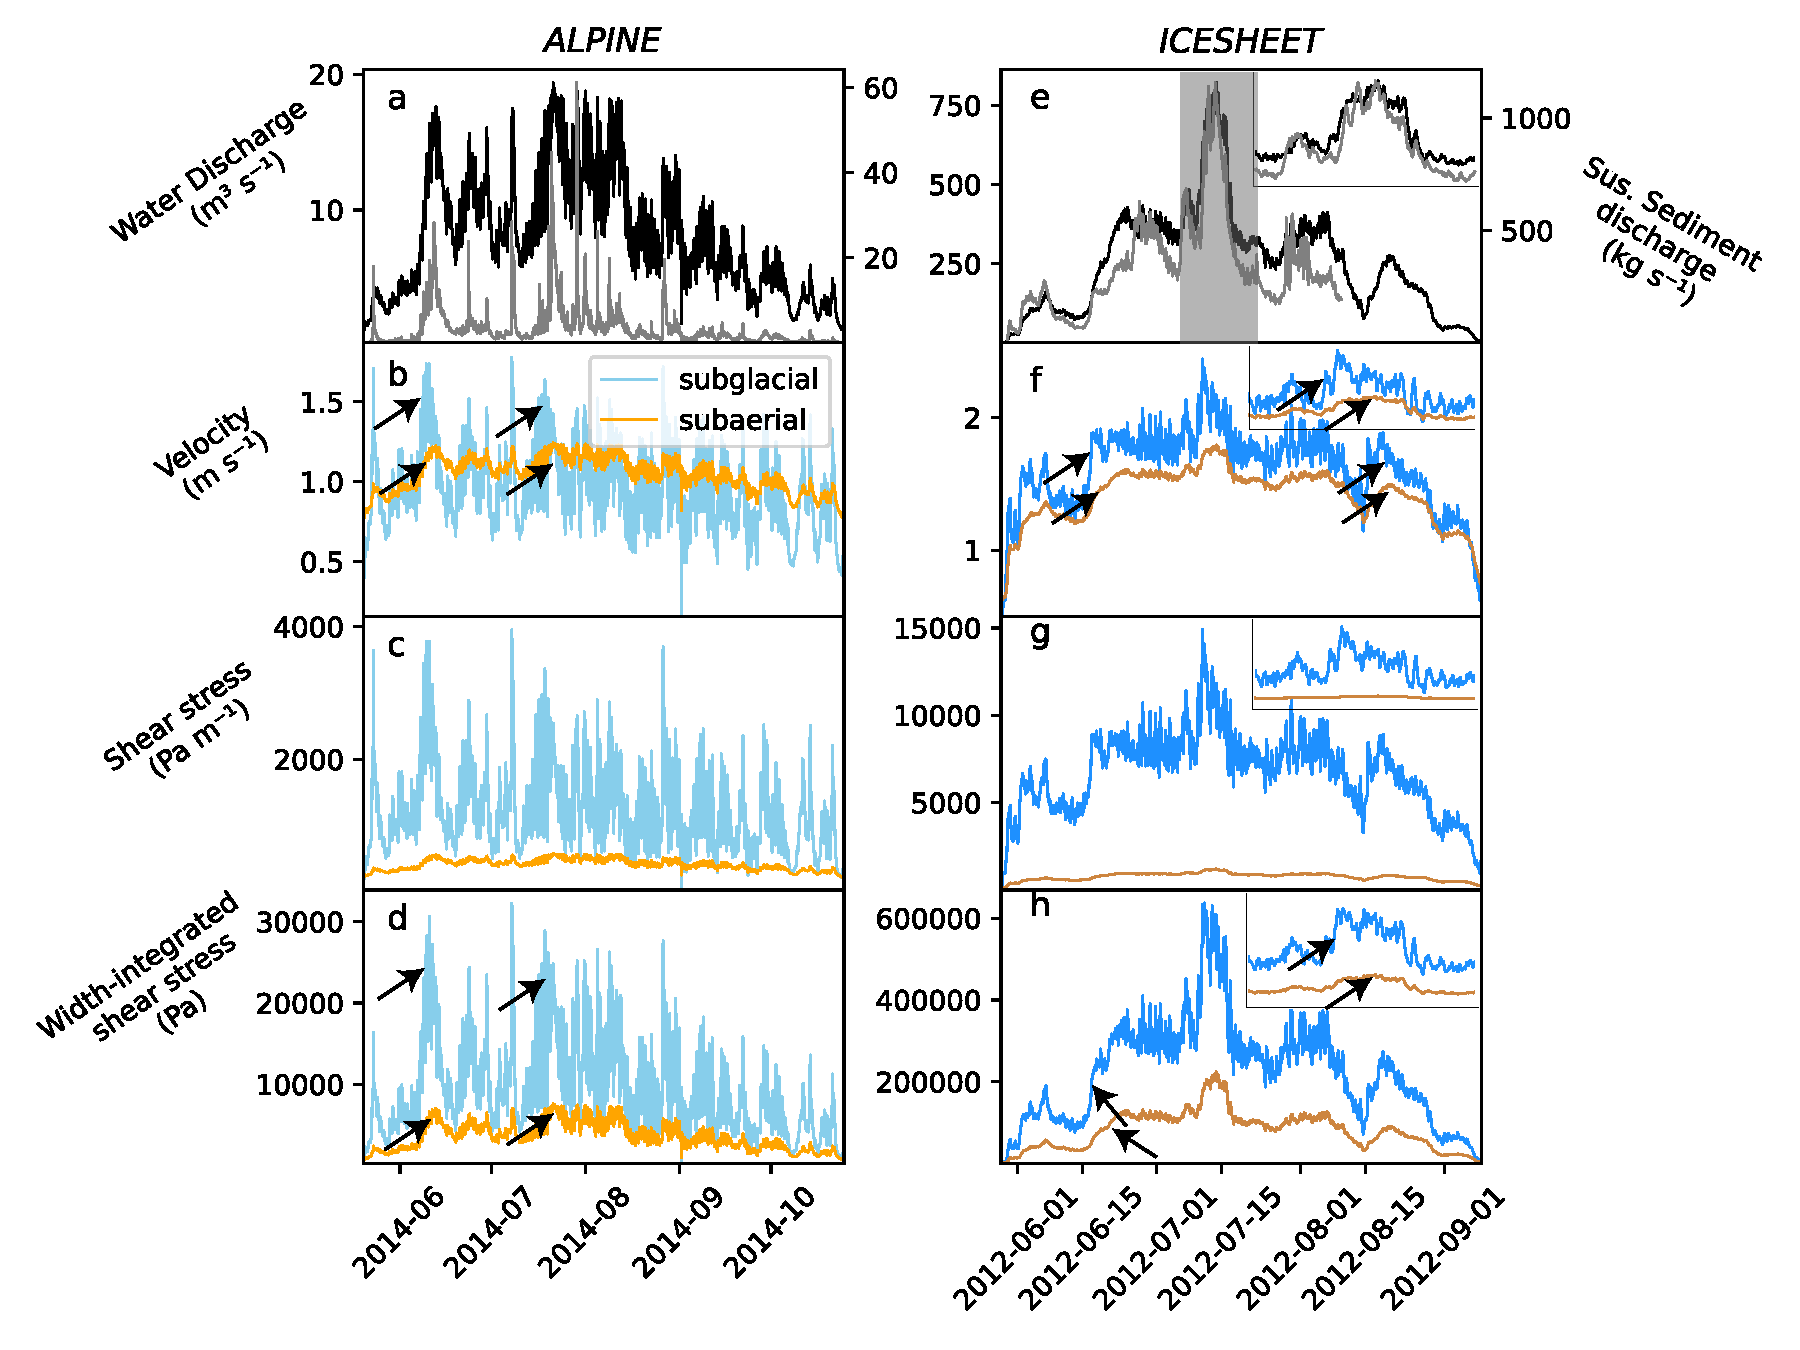
\includegraphics[width=0.9\linewidth]{Fig2.png}
  \caption{Model outputs from simulations using the hydrographs in panels a and e for the scenarios \alpine{} (a-d) and \icesheet{} (e-h).
    Black (gray) lines in a and e represent the subglacial channel size (water discharge).
    Blue (orange) lines represent outputs from the subglacial (subaerial) channel.
    Data are shown at $15$\unit{min} intervals.
    Arrows show examples where variables peak in the subglacial channel before the subaerial one.
    Insets in f-h show the  peak melt event denoted by the shaded area in panels e--h, with an arbitrary y-axis.
  }
  \label{fig:model_outs}
\end{figure}

Conversely, the history dependence on channel size in subglacial channels means that different sediment transport characteristics, such as velocity, occur across a large range of water discharges.
For instance, in subglacial channels in \alpine{},  high water velocity values and shear stresses can occur from a low water discharge  ($\sim\,4$\,\unit{m}$^3$\,\unit{s}$^{-1}$) to the maximum water discharge at over $17$ \,\unit{m}$^3$\,\unit{s}$^{-1}$ (Figure~\ref{fig:Qw_vari}\,a).
In \icesheet{}, water velocities close to the seasonal mean value can occur at water discharges between roughly $150$ \,\unit{m}$^3$\,\unit{s}$^{-1}$ and $310$ \,\unit{m}$^3$\,\unit{s}$^{-1}$.
When considering the subglacial channel's evolving width, width-integrated shear stress across the channel generally increases with water discharge, with improved rank correlation compared to water velocity or shear stress (\alpine{}, Figure~\ref{fig:Qw_vari} a--c).
Yet even the width-integrated shear stress  can vary substantially, with the highest values occurring at water discharge values ranging from roughly $11$ \,\unit{m}$^3$\,\unit{s}$^{-1}$ to over $17$ \,\unit{m}$^3$\,\unit{s}$^{-1}$.
The variability in width-integrated shear stress is less pronounced in the \icesheet{} scenario, where the hydrograph has less diurnal variability (Figure~\ref{fig:Qw_vari} c, f).

\begin{figure}[hbt!]
  \centering
  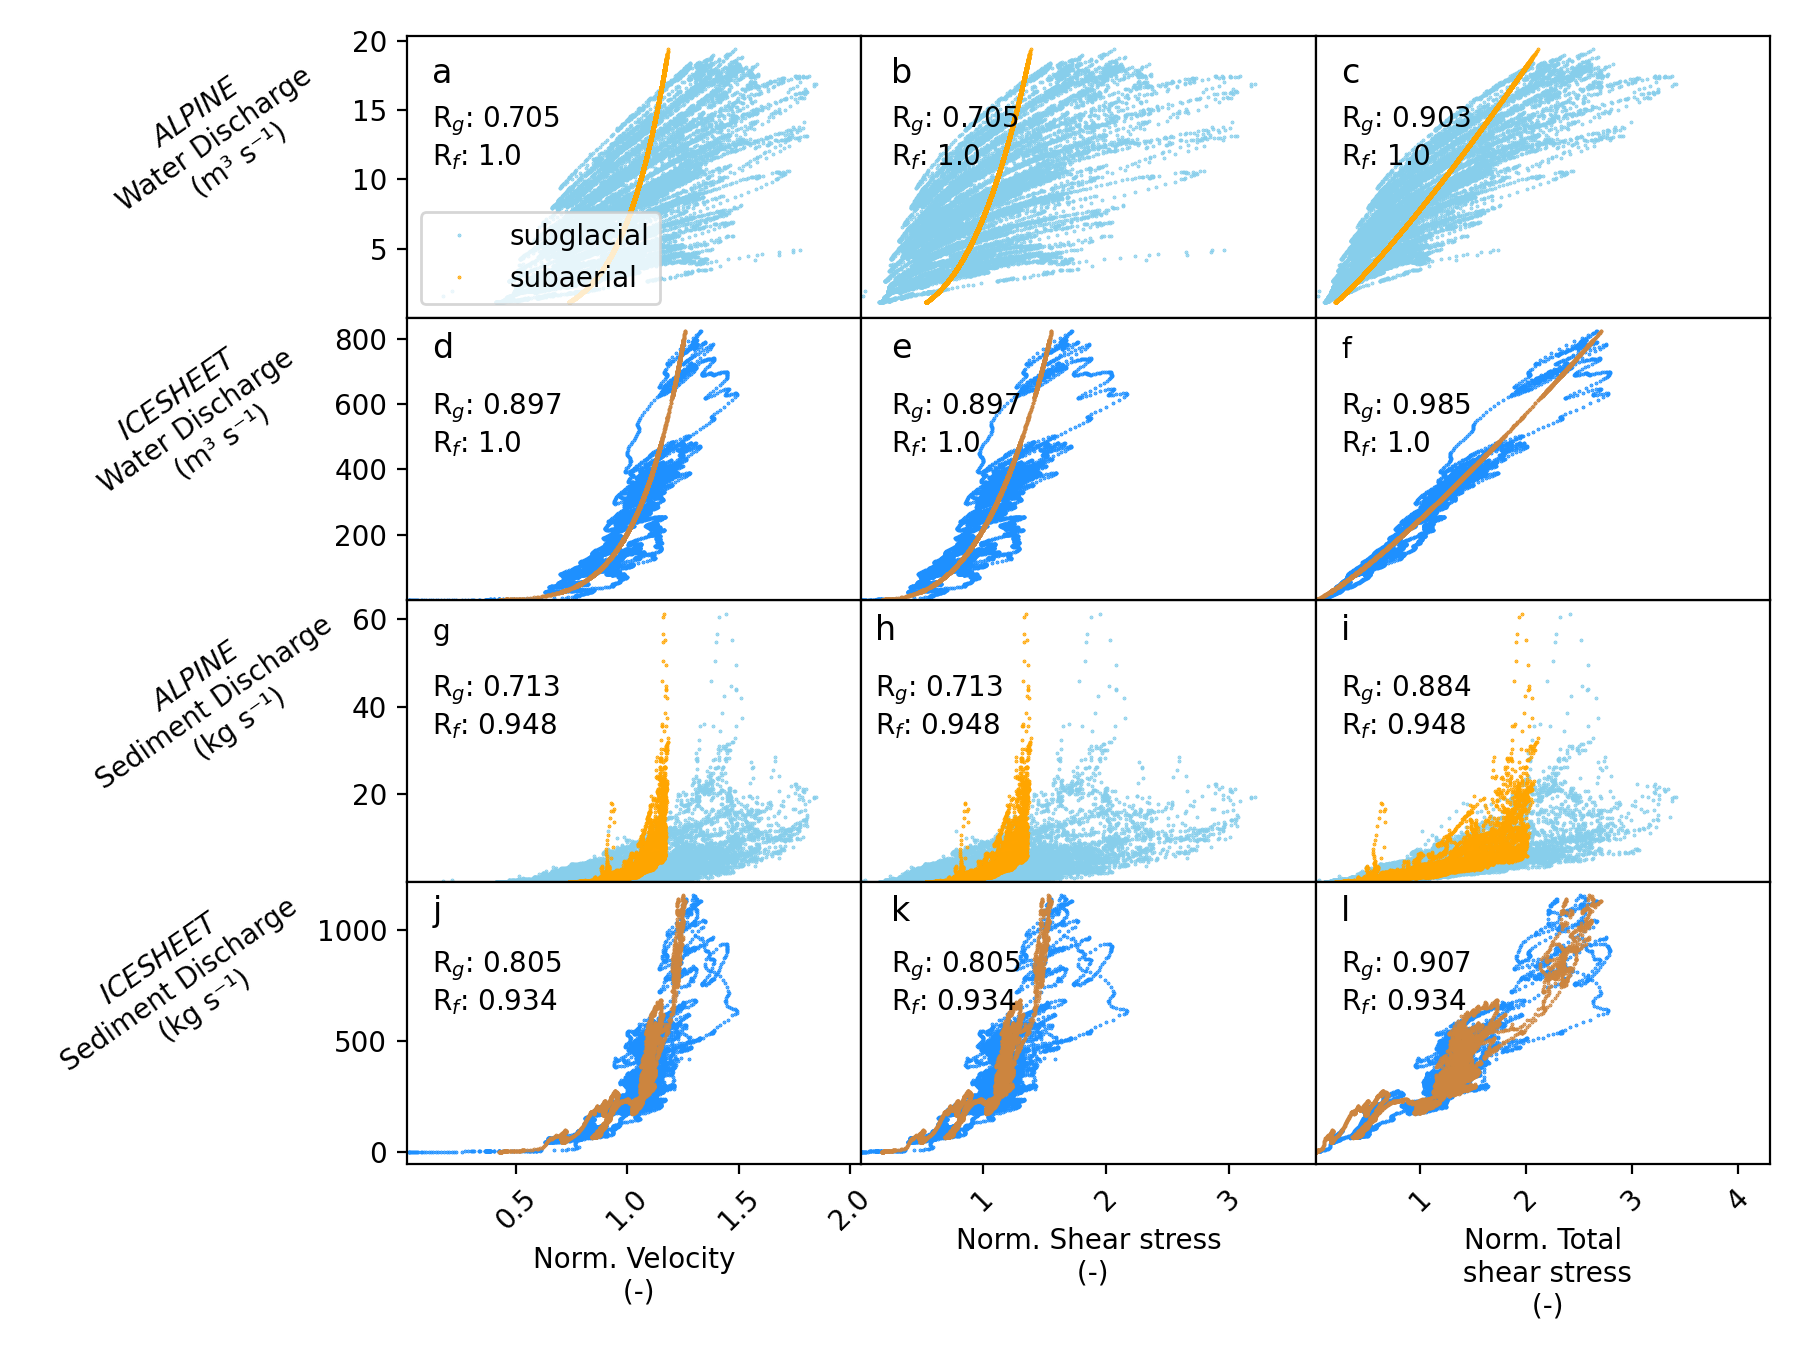
\includegraphics[width=0.9\linewidth]{Fig3.png}
  \caption{
    Relationship between water discharge and normalized velocity, shear stress, and width-integrated shear stress for \alpine{} (a-c) and \icesheet{} (d-f).
    Variables on the x-axis have been normalized to mean values.
    $R_g$ ($R_f$) shows the Spearman rank correlations for the subglacial (subaerial) outputs.
    Plots are shown with discharge and outputs at $15$\unit{min} intervals.
  }
  \label{fig:Qw_vari}
\end{figure}

The different response of subaerial and subglacial model outputs to water discharge impacts the timing of peaks in sediment transport capacity, and thus its  relationship with water discharge.
In the subglacial channel, peaks in $w_g\tau_g$ generally occur when water discharge increases at the fastest rate, but before the maximum water discharge (Figure~\ref{fig:model_outs}\, d and h).
By contrast, in the subaerial channel,   $w_f\tau_f$  peaks when water discharge is highest.

\FloatBarrier
\section{Discussion}

\subsection{Experiment limitations}

Several aspects of the models and  experiment design limit the comparison of the model outputs to field data and make comparison of the two systems difficult.
The lumped nature of the models mean that they operate independently of the upstream drainage network, and sediment access is not considered here.
In reality, processes such as sediment access are highly important in controlling sediment export in glacierized catchments \citep[e.g.][]{herman2015,vergara2022}.
Furthermore, under different glacier configurations and subglacial conditions, new channels can emerge quickly and water can be distributed to flow through several adjacent conduits impacting the sediment transport in each \citep[e.g.][]{werder2013,hewitt2019,delaney2023}.
As a result, these models isolate the relationship between water discharge and sediment transport capacity in subglacial and subaerial systems, making comparison more direct, but neglecting more complex, yet important spatially distributed processes. 

Comparison of model outputs between the subaerial and subglacial case is difficult, given that while the water velocities are comparable in both channel types, the shear stresses and width-integrated shear stresses are much smaller in subaerial channels (Figure~\ref{fig:model_outs}).
This occurs due to the different gradients in the two systems, with the subglacial one being much steeper \citep{alley1997}.
We note, however, that in the ensemble runs in Section~\ref{sect:ensemble}, the range of parameters tested cover the range of viable shear stresses in both subglacial and subaerial channels.

Width-integrated shear stress is examined in the two numerical experiments as it does not have a dependence on grain-size, unlike sediment transport relationships, such as \citet[][Section \ref{sect:scaling}]{meyer1948}.
This makes comparison between the two systems simpler. 
Preferential transport of smaller sediment clasts and the input of upstream sediment impacts sediment transport capacity as grain-size evolves \citep[e.g.][]{gomez1983}.
These processes are only beginning to be evaluated below glaciers \citep{aitken2024}, but can be important in subaerial systems.
Subglacial sorting processes could be an additional source of variability in sediment export from glacier with respect to water discharge, especially with respect to bedload.

\subsection{Increased variability in  sediment transport capacity in subglacial systems}
\label{sect:dis_qsc}

Increased variability in subglacial sediment discharge capacity could make it more difficult to differentiate the role of long-term climatic controls on sediment transport with shorter-term hydrological variations.
In sediment transport relationships that evaluate sediment discharge capacity, such as in \citet{meyer1948} or \citet{engelund1967}, shear stress is scaled to the power of $\frac{3}{2}$ or $\frac{5}{2}$, respectively (Section~\ref{sect:scaling}).
The exponent greater than $1$ magnifies sediment discharge variability beyond the variable sediment transport parameters described above (Figure~\ref{fig:multi_run}; Table~\ref{tab:Qs}).
As a result, the different response to water discharge variations in  shear stress in subglacial channels compared to subaerial ones (Figure~\ref{fig:Qw_vari}) may actually cause even greater variations in sediment transport capacity in subglacial channels than presented above.



Greater variations in subglacial sediment transport capacity compared to subaerial ones could cause a supply-limited regime at many glaciers \citep{alley1997}.
In subglacial systems, sediment's critical shear stress, or threshold at which sediment mobilization occurs, can be reached more frequently and across a range of water discharges, compared to subaerial systems (Figure~\ref{fig:Qw_vari}).
This result suggests sediment export here is especially sensitive to observed changes in water discharge variability, in addition to quantity \citep{lane2019b}.
Sediment exhaustion through repeated crossing of the mobilization threshold may explain the stronger dependence of sediment discharge from the Greenland Ice Sheet on basal shear stress, a proxy for bedrock erosion, rather than glacier melt \citep{overeem2017}.
The repeated crossing of the mobilization threshold across a range of discharges could also result in sediment discharge's strong dependence on sediment production from sliding in many cases \citep{herman2015,koppes2015}.

While transport-limited states below glaciers are likely rare \citep[e.g.][]{alley1997}, they can be possible \citep[e.g.][]{swift2005} and abundant sediment can persist below glaciers \citep[e.g.][]{walter2014,stevens2022,delaney2022}.
At these glaciers, the great variability in subglacial sediment transport capacity may make it difficult to link sediment discharge to hydrology, especially when peak events occur \citep{cowan1988,delaney2018}.
As a result, it may prove challenging to establish the impact on sediment transport capacity  of individual extreme events, such as extreme precipitation or melt \citep{lu2022}, given the potential for different channel sizes with the same hydrology forcing.
However, in the case of bedload, the signal of this variable subglacial sediment transport relationship may be destroyed only a short distance downstream as subaerial hydraulics controls these sediment transport \citep{mancini2023}.

Catchments with reduced water discharge variability may experience yet less variability in sediment transport capacity, as the two hydrological forcings from \alpine{} and \icesheet{} show different variations in model outputs.
Indeed, the more decoupled and sporadic relationship between model outputs and water discharge in \alpine{} results from the relatively larger discharge variations on daily to weekly timescales (Figure~\ref{fig:Qw_vari}).
This occurs as the evolution of the R-channel's size is slow compared to the variations in water discharge.
Such water discharge variability in \alpine{} may cause shear stress to approach $Q^{2}$in assuming pipe-flow conditions \citep[Section \ref{sect:scaling}; c.f.][]{alley1997}.
Conversely, the reduced variability in water discharge in \icesheet{} may result in the R-channel's size being closer to equilibrium from the smaller variations in water discharge.
In this case, the exponent on water discharge for shear stress is likely less than $2$, but greater than $\frac{4}{5}$ that occurs when the R-channel's size evolves in equilibrium with water discharge (see Section \ref{sect:scaling}).
As a result, there is a stronger relationship between subglacial model outputs and water discharge in \icesheet{} compared to \alpine{} (Figure~\ref{fig:Qw_vari}) and less variability model outputs in the \icesheet case (Figure~\ref{fig:multi_run}).



\subsection{Interpreting sediment transport records from glacierized catchments with respect to water discharge}

A sporadic relationship between subglacial sediment transport capacities and water discharge can occur depending on the subglacial channel size (Figure~\ref{fig:Qw_vari}), limiting the use of water discharge as indicator of sediment discharge capacity in these systems.
As a result, characteristics such as bankfull or effective water discharge  that link geomorphic work to hydro-climatic conditions could have limited meaning in evaluating subglacial sediment transport \citep{wolman1960,lenzi2006}.
A glacier's sediment transport capacity is impacted by the ice thickness controlling the channel closure rate, and the glacier's surface slope, in addition to water discharge and sediment size \citep[Figure~\ref{fig:multi_run}, Section~\ref{sect:sub_mode}; ][]{rothlisberger1972,gimbert2016,stevens2022,walder1994}.
In a supply-limited state, a glacier's sediment discharge record also responds to  sediment availability and bedrock erosion from  water pressure variations and sliding  \citep[e.g. ][]{iverson2012,herman2015,delaney2023}.
As a result, the greater amount of in variability the sediment transport evacuation can make it  difficult to isolate the drives of sediment export with respect to hydrological and glaciological conditions \citep{delaney2024}.
This multitude of processes lies in contrast to many subaerial channels, where transport capacity typically responds to water discharge in addition to sediment size, channel shape,  and hydraulic gradient, that can remain stable over years or longer \citep[Section~\ref{sect:fluv}; e.g.][]{tucker1997}.
Strong correlations between water discharge and sediment export in glacier systems could be indicative of other processes, such as increased sediment access \citep{zhang2022}.
Furthermore observed correlation between water discharge and sediment discharge far downstream of the glacier likely represents subaerial transport processes, especially with respect to bedload \citep{mancini2023}.

The co-varying relationship between sediment discharge capacity and water discharge in  subaerial conditions could be noticeable $\sim20$\,\unit{km} downstream of the Leverett site, where a strong correlation persists between sediment plume size and the river's water discharge into the Kangerlussuaq fjord \citep{chu2009,mcgrath2010}.
In contrast, in marine-terminating glacier catchments, a less consistent relationship may occur between water discharge or melt extent and sediment plume size \citep{chu2012,tedstone2012}.
Here, ocean water pressurizes subglacial channels at the ice front \citep[e.g.][]{how2017}, so the reduced correlation could result from the inconsistent relationship between subglacial sediment transport capacity and water discharge presented here.

Water discharge measurements at the hourly timescale remain unavailable in many catchments, further limiting subglacial  sediment transport models in capturing specific events.
The model output variability in subglacial channels decreases substantially beyond $1-5$ days of smoothing (Figure~\ref{fig:multi_run}).
Over this time period, subglacial channels could be in closer equilibrium conditions with water discharge variations leading to a stronger relationship with sediment discharge capacity (Section ~\ref{sect:scaling}).
Applying water discharge averaged over these time periods omits key sediment discharge characteristics, such as the timing of peaks in sediment transport capacity from glaciers (Figure~\ref{fig:model_outs}), that could play a key role in sediment export from glaciers.
Yet, hydrographs with minimal variability may result in a strong correlation between sediment transport capacity and water discharge, if the water discharge evolves slowly with respect the subglacial channel size.

\conclusions

The sediment transport capacity of a channel is driven by its width and the shear stress exerted by the flowing water, which is proportional to  flow velocity squared.
Subaerial channels alter both their channel width and water velocity immediately in response to changing water discharge.
In contrast, pressurized subglacial channels largely accommodate rapidly changing water discharge by altering water velocity.
Their size responds over several days to changes in discharge.
Thus the response of sediment transport capacity is much more sensitive to changes in water discharge in subglacial channels compared to subaerial ones, although not as variable as if the size of the subglacial conduit was fixed.

With respect to the  manuscript's first objective,
results demonstrate that sediment transport capacity variability is higher in subglacial channels with evolving size across a range of channel shapes and friction factors.
Increased variability even occurs in environments where the water discharge has relatively small diurnal variations, as in the \icesheet case.
The role of this increased noise in sediment transport capacity in evaluating hydro-climatic signals from sediment records in glacierized catchments needs further evaluation.
Furthermore, this processes may lead to sediment exhaustion by subglacial water repeatedly crossing the mobilization threshold across a range of water discharges. 

The manuscript's second objective is establish if water discharge varies with subglacial sediment transport capacity.
Results here suggest that, even in a transport-limited subglacial system, an incoherent relationship between water and subglacial sediment discharge could be expected.
This presents a challenge in linking hydro-climatic conditions to sediment export from glaciers.
Due to evolving subglacial channel size, the timing of peak sediment discharge capacity in subglacial channels occurs before peak  water discharge, whereas it is coincident in subaerial ones.
Our analysis shows that high correlation between water discharge and sediment transport capacity could be possible when water discharge varies at a slower rate than subglacial channel size.
In natural environments, this is appears to often not be the case, but might be conceivable in very large catchments or ones at high latitudes with muted diurnal variations in melt.

 
Lack of observation of the subglacial environment hindered our ability to quantify processes such as
the shape of subglacial channels, the response time of subglacial channels to water discharge variations, and
subglacial sediment size and sorting processes, linking shear stress to  sediment discharge.
Further quantifying these processes will help to better inform the response of sediment discharge capacity to water discharge forcing in subglacial environments.

This study calls for careful analysis when examining the relationship between sediment transport capacity and hydro-climatic conditions from glacierized catchments, especially ones with high water discharge variability.


\codedataavailability{
Code, with links to the data, can be found at \url{https://bitbucket.org/IanDelaney/xsection/src/master/}.
Data from Leverett glacier have been previous published in \citet{tedstone2013}.
Data from Fiescher glacier have been previous published in \citet{delaney2024}.
Code will be uploaded to a permanent repository, with FAIR principles pending acceptance of the paper.}


\authorcontribution{
I.D. designed the study, developed, and implemented the model and experiments, and wrote the manuscript.
A.J.T. helped interpret data from Leverett Glacier and provided guidance on experiment design.
M.A.W. provided data from Fieschergletscher and added the relationship between shear stress and water discharge (see Section \ref{sect:scaling}).
D.F. provided data from Fieschergletscher.
All authors provided key inputs in writing and editing the manuscript.} %% this section is mandatory

\competinginterests{The authors declare no competing interests.} %% this section is mandatory even if you declare that no competing interests are present



\begin{acknowledgements}
SNSF Project No. $\mathrm{PZ00P2}$\_$202024$ provided  funding for I. Delaney.
A. Tedstone acknowledges funding from the European Research Council, award $818994$ -- CASSANDRA.
G. King and M. J. Gevers provided useful comments on a previous version of this manuscript.
We benefited from fruitful discussions with J. Irving.
We thank three reviewers for constructive and critical reviews on a previous version of the manuscript.
\end{acknowledgements}
\newpage

\appendix
\appendixtables   %% needs to be added in front of appendix tables
\begin{table}
  \caption{As Table~\ref{tab:Qs} but with the fractional exponents stated as rounded decimal numbers.  For the subaerial regime the exponents are for displayed for the likely width-exponent $\alpha=1$, as well as its end members 0 (slot canyon) and 1 (only width increases and not depth).
  }
  \small
  \label{tab:Qs2}
  \begin{tabular}{lllll}
    & Width \(\times \,\, \tau\) & MPM & EH & Bagnold\\
    & \(w\, \tau\) & \(Q_s \propto w\, \tau^{3/2}\) & \(Q_s \propto w\, \tau^{5/2}\) & \(Q_s \propto w^{-1/2}\, \Omega^{3/2} H^{-2/3}\)\\
    \hline
    Subaerial (\(\alpha=0\)) & \(f^{0.7}\, Q^{0.7}\,  \Psi^{0.7}\) & \(f^{0.5}\, Q \,\,\,\, \Psi\) & \(f^{0.8}\, Q^{1.7} \, \Psi^{1.7}\) & \(f^{-0.2}\, Q^{1.1} \, \Psi^{1.7}\)\\
    Subaerial (\(\alpha=0.3\)) & \(f^{0.7}\, Q^{0.8}\,  \Psi^{0.7}\) & \(f^{0.5}\, Q \,\,\,\, \Psi\) & \(f^{0.8}\, Q^{1.3} \, \Psi^{1.7}\) & \(f^{-0.2}\, Q^{1.0} \, \Psi^{1.7}\)\\
    Subaerial (\(\alpha=0.5\)) & \(f^{0.7}\, Q^{0.8}\,  \Psi^{0.7}\) & \(f^{0.5}\, Q \,\,\,\, \Psi\) & \(f^{0.8}\, Q^{1.3} \, \Psi^{1.7}\) & \(f^{-0.2}\, Q^{1.0} \, \Psi^{1.7}\)\\
    Subaerial (\(\alpha=1\)) & \(f^{0.7}\, Q^{1.0}\,  \Psi^{0.7}\) & \(f^{0.5}\, Q \,\,\,\, \Psi\) & \(f^{0.8}\, Q^{0.7} \, \Psi^{1.7}\) & \(f^{-0.2}\, Q^{1.0} \, \Psi^{1.7}\)\\[3pt]
    R-channel & \(f^{0.4}\, Q^{0.8} \, \Psi^{0.6}\) & \(f^{0.5}\, Q \,\,\,\, \Psi\) & \(f^{0.7}\, Q^{1.4}\, \Psi^{1.8}\) & \(f^{-0.2}\, Q^{1.0} \, \Psi^{1.7}\)\\
    Pipe & \(f \,\quad Q^{2\phantom{.0}} \, S^{-1}\) & \(f^{1.5}\, Q^3 \, S^{-2.5}\) & \(f^{2.5}\, Q^{5\phantom{.0}}\, S^{-4.5}\) & \(f^{1.5} \,\,\,\,\, Q^{4.5} \, S^{-4.7}\)\\
  \end{tabular}
\end{table}



%\appendixfigures  %% needs to be added in front of appendix figures

%

%% Please add \clearpage between each table and/or figure. Further guidelines on figures and tables can be found below.




\bibliographystyle{copernicus}
\bibliography{Paperlib.bib}


%% REFERENCES

%% The reference list is compiled as follows:

% \begin{thebibliography}{}

% \bibitem[AUTHOR(YEAR)]{LABEL1}
% REFERENCE 1

% \bibitem[AUTHOR(YEAR)]{LABEL2}
% REFERENCE 2

% \end{thebibliography}

%% Since the Copernicus LaTeX package includes the BibTeX style file copernicus.bst,
%% authors experienced with BibTeX only have to include the following two lines:
%%
%% 
%% \bibliography{example.bib}
%%
%% URLs and DOIs can be entered in your BibTeX file as:
%%
%% URL = {http://www.xyz.org/~jones/idx_g.htm}
%% DOI = {10.5194/xyz}


%% LITERATURE CITATIONS
%%
%% command                        & example result
%% \citet{jones90}|               & Jones et al. (1990)
%% \citep{jones90}|               & (Jones et al., 1990)
%% \citep{jones90,jones93}|       & (Jones et al., 1990, 1993)
%% \citep[p.~32]{jones90}|        & (Jones et al., 1990, p.~32)
%% \citep[e.g.,][]{jones90}|      & (e.g., Jones et al., 1990)
%% \citep[e.g.,][p.~32]{jones90}| & (e.g., Jones et al., 1990, p.~32)
%% \citeauthor{jones90}|          & Jones et al.
%% \citeyear{jones90}|            & 1990



%% FIGURES

%% When figures and tables are placed at the end of the MS (article in one-column style), please add \clearpage
%% between bibliography and first table and/or figure as well as between each table and/or figure.

% The figure files should be labelled correctly with Arabic numerals (e.g. fig01.jpg, fig02.png).


%% ONE-COLUMN FIGURES

%%f
%\begin{figure}[t]
%\includegraphics[width=8.3cm]{FILE NAME}
%\caption{TEXT}
%\end{figure}
%
%%% TWO-COLUMN FIGURES
%
%%f
%\begin{figure*}[t]
%\includegraphics[width=12cm]{FILE NAME}
%\caption{TEXT}
%\end{figure*}
%
%
%%% TABLES
%%%
%%% The different columns must be seperated with a & command and should
%%% end with \\ to identify the column brake.
%
%%% ONE-COLUMN TABLE
%
%%t
%\begin{table}[t]
%\caption{TEXT}
%\begin{tabular}{column = lcr}
%\tophline
%
%\middlehline
%
%\bottomhline
%\end{tabular}
%\belowtable{} % Table Footnotes
%\end{table}
%
%%% TWO-COLUMN TABLE
%
%%t
%\begin{table*}[t]
%\caption{TEXT}
%\begin{tabular}{column = lcr}
%\tophline
%
%\middlehline
%
%\bottomhline
%\end{tabular}
%\belowtable{} % Table Footnotes
%\end{table*}
%
%%% LANDSCAPE TABLE
%
%%t
%\begin{sidewaystable*}[t]
%\caption{TEXT}
%\begin{tabular}{column = lcr}
%\tophline
%
%\middlehline
%
%\bottomhline
%\end{tabular}
%\belowtable{} % Table Footnotes
%\end{sidewaystable*}
%
%
%%% MATHEMATICAL EXPRESSIONS
%
%%% All papers typeset by Copernicus Publications follow the math typesetting regulations
%%% given by the IUPAC Green Book (IUPAC: Quantities, Units and Symbols in Physical Chemistry,
%%% 2nd Edn., Blackwell Science, available at: http://old.iupac.org/publications/books/gbook/green_book_2ed.pdf, 1993).
%%%
%%% Physical quantities/variables are typeset in italic font (t for time, T for Temperature)
%%% Indices which are not defined are typeset in italic font (x, y, z, a, b, c)
%%% Items/objects which are defined are typeset in roman font (Car A, Car B)
%%% Descriptions/specifications which are defined by itself are typeset in roman font (abs, rel, ref, tot, net, ice)
%%% Abbreviations from 2 letters are typeset in roman font (RH, LAI)
%%% Vectors are identified in bold italic font using \vec{x}
%%% Matrices are identified in bold roman font
%%% Multiplication signs are typeset using the LaTeX commands \times (for vector products, grids, and exponential notations) or \cdot
%%% The character * should not be applied as mutliplication sign
%
%
%%% EQUATIONS
%
%%% Single-row equation
%
%\begin{equation}
%
%\end{equation}
%
%%% Multiline equation
%
%\begin{align}
%& 3 + 5 = 8\\
%& 3 + 5 = 8\\
%& 3 + 5 = 8
%\end{align}
%
%
%%% MATRICES
%
%\begin{matrix}
%x & y & z\\
%x & y & z\\
%x & y & z\\
%\end{matrix}
%
%
%%% ALGORITHM
%
%\begin{algorithm}
%\caption{...}
%\label{a1}
%\begin{algorithmic}
%...
%\end{algorithmic}
%\end{algorithm}
%
%
%%% CHEMICAL FORMULAS AND REACTIONS
%
%%% For formulas embedded in the text, please use \chem{}
%
%%% The reaction environment creates labels including the letter R, i.e. (R1), (R2), etc.
%
%\begin{reaction}
%%% \rightarrow should be used for normal (one-way) chemical reactions
%%% \rightleftharpoons should be used for equilibria
%%% \leftrightarrow should be used for resonance structures
%\end{reaction}
%
%
%%% PHYSICAL UNITS
%%%
%%% Please use \unit{} and apply the exponential notation


\end{document}


% \ian{comeback here}
% For sufficiently short periods, channel width and wetted area are fixed in the subglacial system (akin to pipe flow) so that the response of width-integrated shear stress is $w_g\, \tau_{g}\, \propto\,  Q^{2}$ \citep[Table\,~\ref{tab:Qs}; ][]{alley1997}.

% R\"othlisberger channels in steady state with water discharge (i.e. channel sizes evolves at a faster rate than water discharge), the width-integrated shear stress response to water discharge is $ w_g\,\tau_{g}\, \propto\,  Q^{\sim\frac{4}{5}}$ (Table\,~\ref{tab:Qs}).
% This relationship suggests that when discharge varies more slowly than channel shape subglacial channels have less variable sediment transport capacity than subaerial ones.
% Yet, subglacial channels rarely operate in a steady state \citep{gimbert2016}.
% However, the reduced variability in the  \icesheet{} case compared to the \alpine{} one suggests that it is closer to an equilibrium state (Figure~\ref{fig:Qw_vari}).
% \ian{comeback here}
% The channel width and size variations in subglacial channels presented here also occur in subaerial channels in response to water discharge \citep{phillips2016}, likely over decadal timescales or in response to individual extreme events \citep{slater2013,dean2013}.
% These timescales are considerably longer than the continuous changes to the subglacial channel's response time of days.
% Even so, if channel width changes occur in subaerial channels, then the values of $\alpha$ in Equation~\ref{eq:wcf} could change in time.
% $\alpha$ must be less than $1$, and even this would cause the exponent on $Q$ in the  $w_g\,\tau_{g}$ relationships to remain substantially below that of pipeflow (see Sections \ref{sect:scaling}, Table~\ref{tab:Qs}, Figure~\ref{fig:multi_run}).

With even smaller water discharge variations, the subglacial sediment transport capacity may behave similarly to the subaerial system.
Note that in pipe flow conditions, maximum sediment transport would coincide with peak water discharge, unlike the evolving channel size alters the timing (Figure \ref{fig:model_outs} and \ref{fig:Qw_vari}).